\chapter{原子核的结合能与液滴模型}

\section{原子核的结合能}

\subsection{质量与能量的一般关系}

\textbf{质能方程:}$E=mc^2$

相对论还给出,以速度数值$v$运动的粒子为例,其中$m_0$是粒子的静止质量。当粒子的速度v增大时,它的质量$m$也随之增大。

$$ m = \frac{m_0}{\sqrt{ 1 - (\frac{v}{c})^2}} $$

总能量$E$ = 静止质量$m_0c^2$ + 动能$E_k$,即$E=m_0c^2 + E_k$

对于光子来说,静止质量为零,但有动能。光子的总能量等于它的动能。

\textbf{质量亏损:}组成某一原子核的所有核子质量和与该原子核质量的差称为原子核的质量亏损。

\textbf{广义质量亏损:}体系变化前后静止质量之差。

\textbf{原子核的结合能:}自由核子组成原子核时放出的能量或原子核分解为自由核子时吸收的能量,都叫原子核的结合能,它是原子核整体稳定性的度量。

例如,一个中子和一个质子结合成氘核时,要放出2.22兆电子伏的能量,这个能量以$\gamma$光子的形式辐射出去。

\textbf{比结合能:}原子核平均每个核子的结合能又称为比结合能。

比结合能表示,若把原子核拆成自由核子,平均对于每个核子所要做的功。比结合能ε的大小,可以用以标志原子核结合的松紧程度。越大的原子核结合的越紧;越小的原子核结合的较松。比结合能的物理意义是将原子核拆散成自由核子时,外界对每个核子所做的最小的平均功。

\textbf{$\beta$稳定线:}原子核靠核力和库仑力维持平衡,核力是核子之间都有的,库仑力只在质子中有,随着质子数的增加,库仑力增加,这时候还要维持平衡的话,就不能添加质子,只能添加中子了,因为添加中子会增加核力,但不增加库仑力。这也解释了$\beta$稳定线在质子比较大的领域,$N>Z$,其中$^{208}Pb$的中质比$\frac{N}{Z}=1.54$

\textbf{核子数的稳定性:}自然界接近300种稳定核中,偶偶核更稳定。如图~\ref{fig003}~所示。

\begin{figure}[htbp]
    \centering
    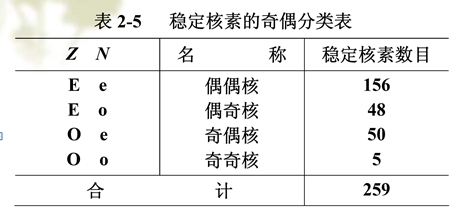
\includegraphics[width=10cm]{figure//fig003.png}
    \caption{\label{fig003}稳定核素的奇偶分类表。}
\end{figure}

\textbf{重核的不稳定性:}实验发现,能发生$\alpha$衰变的天然放射性核素都是一些重核,其中最轻的是$^{142}Ce$,很重的核几乎都具有$\alpha$放射性。能够发生自发裂变的核素也都是些很重的核。

\section{液滴模型}

液滴模型来自于比结合能曲线。

\textbf{结合能的半经验公式:}$B=B_V + B_S + B_C + B_{sym} + B_P$

\begin{itemize}
    \item $B_V$为体积能。
    \item $B_S$为表面能。
    \item $B_C$为库伦能。
    \item $B_{sym}$为对称能。
    \item $B_P$为对能。
\end{itemize}

比结合能各项的贡献如图~\ref{fig004}~所示。

\begin{figure}[htbp]
    \centering
    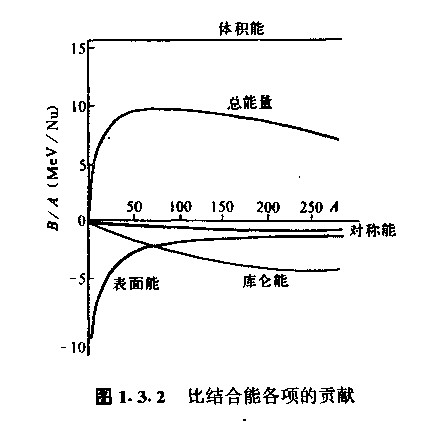
\includegraphics[width=8cm]{figure//fig004.png}
    \caption{\label{fig004}比结合能各项的贡献。}
\end{figure}

根据液滴模型,可以推出$\beta$稳定线,其为比结合能的极值点。也能推出中子滴线、质子滴线,其为比结合能为0的点。